\begin{figure*}[htbp]
    \centerline{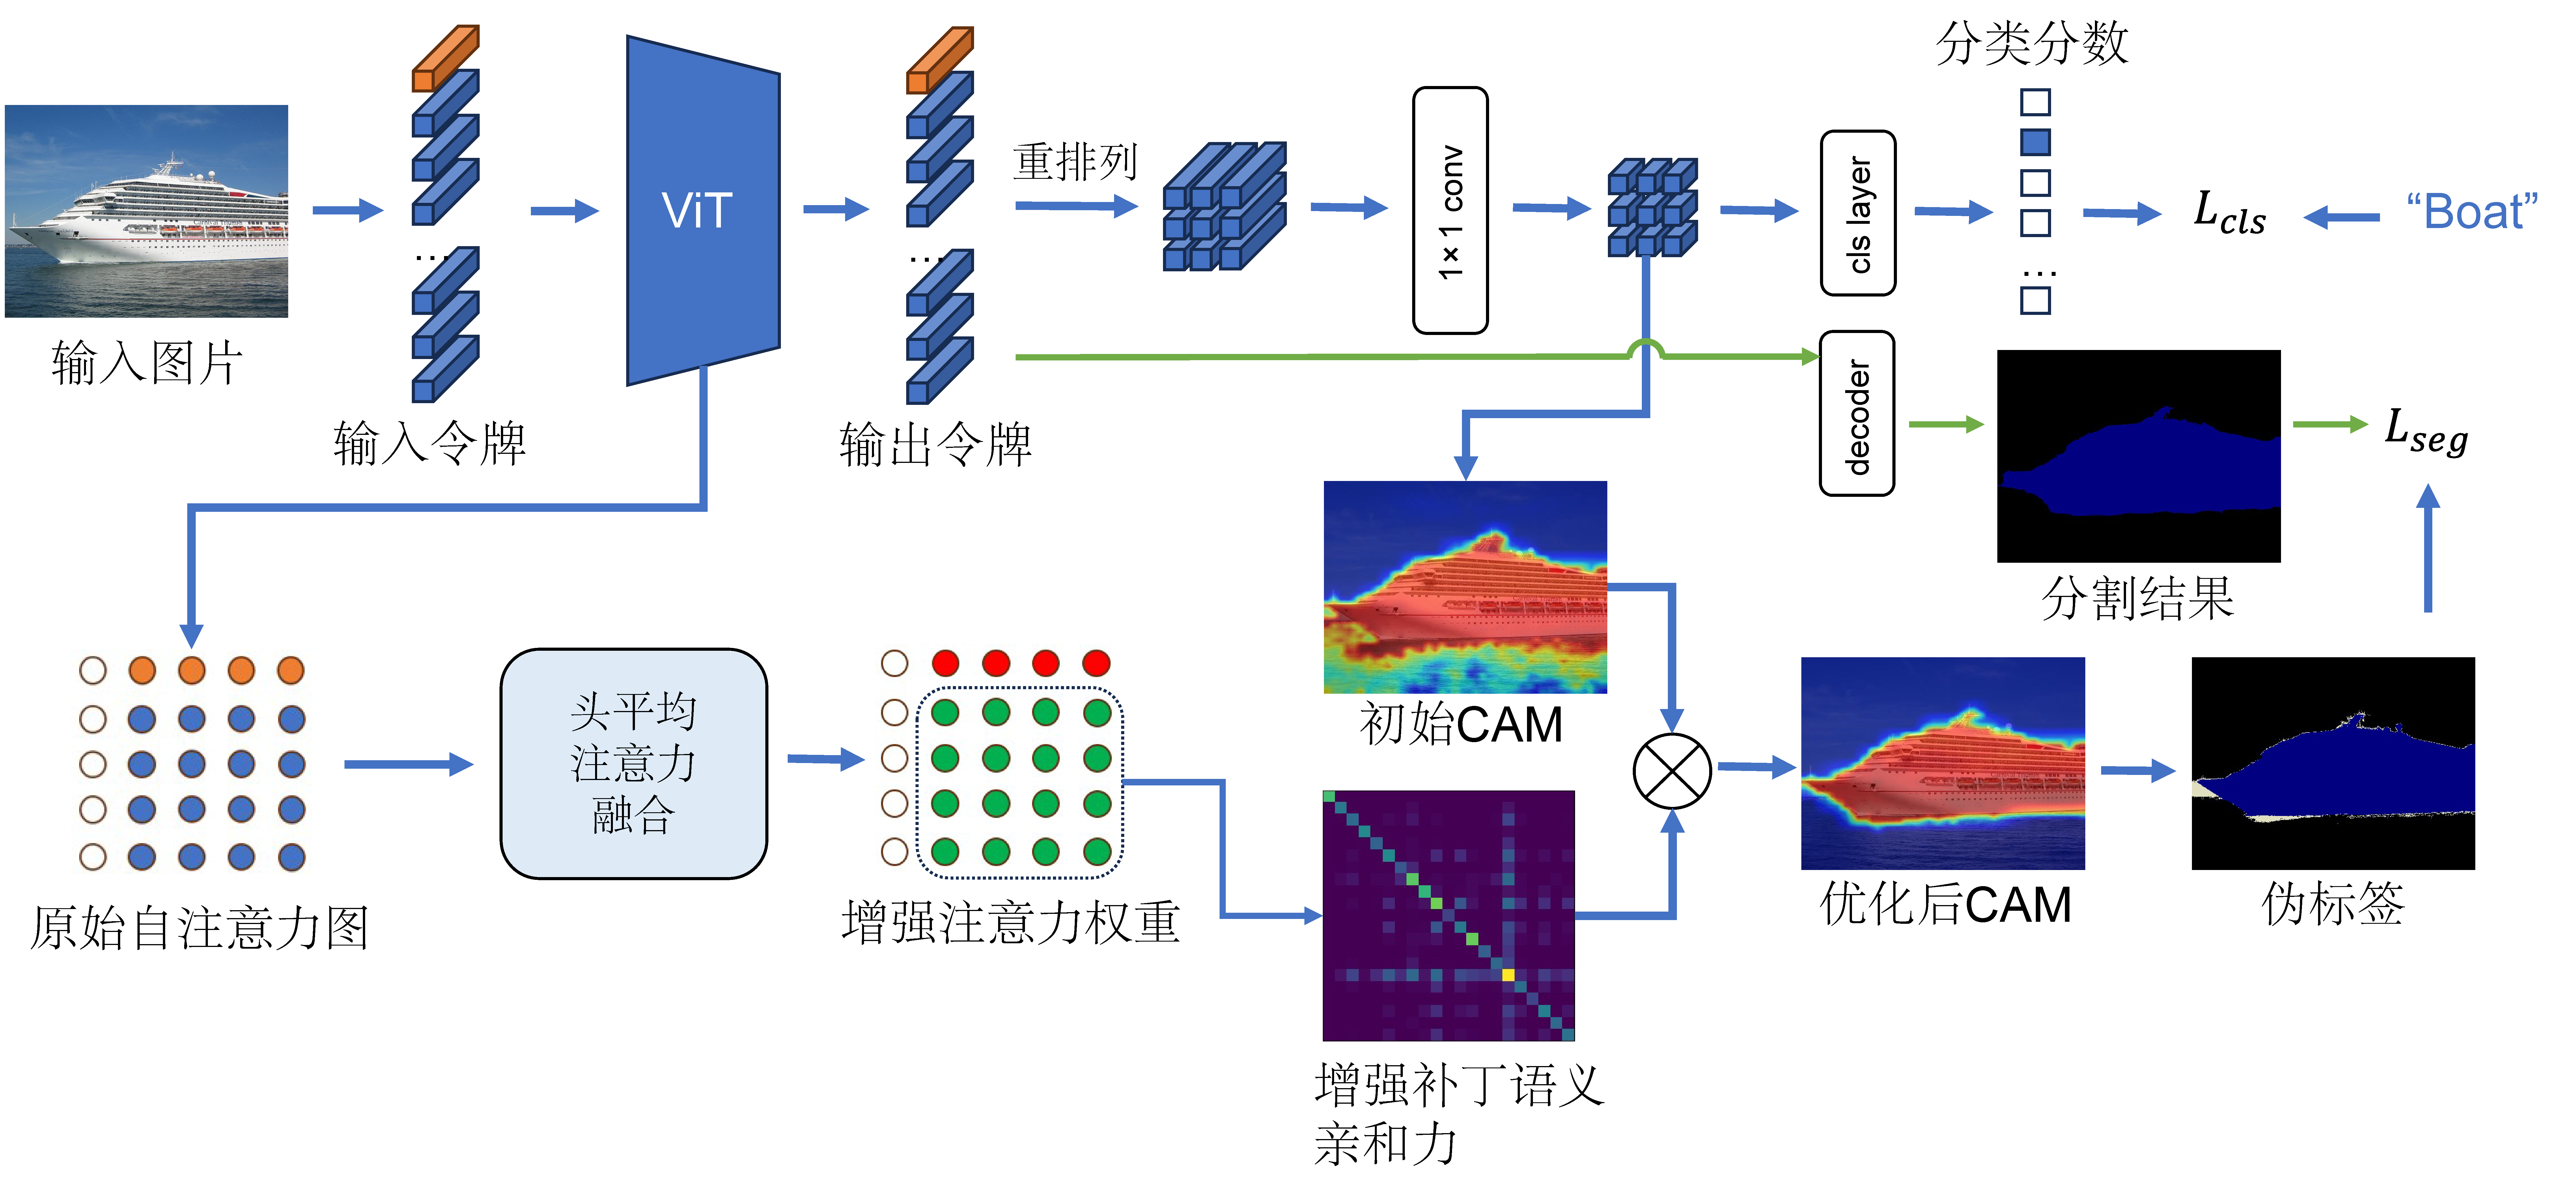
\includegraphics[width=6in]{fig/fig1.pdf}}
    \begin{CJK*}{UTF8}{fs}
        \caption{SS-EPA整体框架。SS-EPA首先将输入图像分成多个补丁,每个补丁线性转换成补丁令牌,并连接一个类别令牌。ViT输出令牌一方面经过重拍列和$1\times 1$卷积生成初始CAM,并由分类层输出分类分数。另一方面经过分割decoder生成语义分割结果。然后从ViT中提取多头自注意力图,并通过HAAF模块进行增强,获取增强补丁语义亲和力。最后通过增强补丁语义亲和力对初始CAM进行优化,并生成伪标签用于监督分割任务。}\label{fig1}
    \end{CJK*}
\end{figure*}

\begin{CJK*}{UTF8}{zhhei}
    \zihao{5}
    \vskip 1mm
    \section{引言}
\end{CJK*}

\begin{CJK*}{UTF8}{fs}
    深度学习推动图像分割显著进步,但依赖精确标注样本,成本高昂。弱监督语义分割(WSSS)技术因此出现,WSSS仅需粗略标注的样本,大幅降低了样本获取的难度。弱监督标注分为边框级标注\cite{39dai2015boxsup,40zhang2021affinity}、涂鸦级标注\cite{41lin2016scribblesup}和图像级标\cite{03ru2023token,12xu2022multi}。其中最难利用的是图像级标注,因为它通常只提供图片的分类标签,包含极少可利用的语义信息,也是多数研究人员最热衷于研究的方法之一。本工作只使用图像级弱标注。

	先前的WSSS方法通常采用多阶段方法,即先训练一个分类网络来生成类激活图Class Activation Map(CAM)\cite{01zhou2016learning},获取类别在图像中的位置信息。然后通过扩展优化CAM生成伪标签,最后利用伪标签全监督地训练语义分割模型。虽然多阶段方法通常可以获得更精准的CAM和更优秀的分割性能,但通常需要分阶段地训练模型和不同的训练策略,耗费大量的计算资源和时间来进行训练和优化,这限制了其在大规模数据集或实时应用中的实用性。通过CNN生成的CAM,存在只激活最显著区域的缺点,原因是CNN感受野有限,对全局信息捕获不完善。Vision Transformer(ViT)\cite{02dosovitskiy2020image}在其它视觉任务中的巨大成功,引起了WSSS领域研究人员的广泛关注\cite{03ru2023token,12xu2022multi,13ru2022learning}。ViT是一种基于 Transformer 架构的视觉模型,它将输入图片划分为小的补丁(patch),并利用Transformer 来建模这些补丁之间的关系。且ViT采用无卷积架构,避免了卷积带来的先验约束,如局部性和平移不变性,使ViT具有更好的可扩展性。基于ViT的WSSS方法首先通过补丁令牌生成粗略的初始CAM,再利用多头自注意力中包含的语义亲和力信息对初始CAM进行优化\cite{12xu2022multi}。然而Transformer中不同深度层的多头自注意力可能关注不同部分,如浅层更关注局部结构、纹理颜色等,深层能捕获更广泛和抽象的视觉语义信息,直接将其与CAM相乘可能会产生错误与误导。且ViT注意力图十分庞大,直接提取所有注意力权重会占据大量计算资源。

	本文提出一种单阶段 WSSS 方法 SS-EPA (Single Stage WSSS with Enhanced Patch Affinity) ,和一种头平均注意力融合增强模块 (Head Average Attention Fusion,HAAF) 。针对先前 CAM 优化多数集中在多阶段方法上的问题,本文提出一种单阶段 WSSS 方法 SS-EPA ,集成了端到端式多头自注意力 CAM 优化方法。 SS-EPA 从 ViT 的自注意力中提取补丁语义亲和力信息,并用于优化初始 CAM 。本文将该端到端的优化方法集成到单阶段 WSSS 方法中,不会影响其完整性和一致性。针对注意力图较为庞大,且不同深度的注意力特性各不相同的问题,本文提出一种头平均注意力融合增强模块 HAAF 。 HAAF 对来自不同层多头自注意力中的语义亲和力进行融合增强,并用于优化从 Transformer 生成的 CAM 。 HAAF 通过对多头自注意力中的各头权重进行平均,聚合不同语义信息,减少不同头重复关注相似区域的冗余信息。随后,通过全局平均池化聚合每个注意力图的全局特征,并将其输入多层感知机,提取更复杂的特征关系。最终获得融合后的增强注意力图,充分考虑了不同层次注意力的重要性。 HAAF 可以去除头重复关注、包含无效信息的冗余问题,显著降低计算资源消耗并提升效率。该方法还能减少每个头对噪声或异常的敏感度,提高模型鲁棒性。

	为了验证本文提出的 SS-EPA 和 HAAF 模块的有效性,本文在 Pascal VOC 2012数据集上评估了SS-EPA的CAM、伪标签和分割结果的性能表现,并与基线方法ToCo\cite{03ru2023token}相比较。对比实验、消融实验以及各种可视化结果表明,本文所提方法可以显著优化生成的CAM,伪标签和分割模型误分类的概率更小,且有更加完整和准确的对象边界。在VOC验证集上与基线相比,伪标签和分割性能分别提升了2.2\%和1.3\%的mIoU分数,充分验证了本文方法的有效性。

    总的来说,本文主要贡献包括以下三个方面:
    \begin{itemize}
        \item 提出了一种名为 SS-EPA 的单阶段 WSSS 方法,集成了端到端式多头自注意力 CAM 优化方法。在不影响单阶段方法的完整性和一致性的前提下,集成了利用补丁语义亲和力信息优化初始 CAM 的方法,使 CAM 更加精细和准确,从而生成更加优质的伪标签用于训练分割模型。
        \item 提出一种头平均注意力融合增强模块(HAAF),来解决语义亲和力信息包含噪声与错误,以及注意力图较为庞大的问题。通过对注意力的不同头的权重做平均,HAAF可去除冗余信息并提高模型鲁棒性,利用多层感知机的交互能力,HAAF可以充分考虑来自不同层注意力的重要性,对包含语义亲和力的自注意力完成简化和增强。
        \item 在 Pascal VOC 2012 数据集上的实验表明,本文方法可以显著优化生成的 CAM ,最终的分割模型性能相比以前的单阶段方法有了实质性的改进,且实现了与一些多阶段方法相当的性能。
    \end{itemize}
\end{CJK*}